\chapter{Multi-task learning}

So far we have considered \ac{AES} and \ac{NLI} as independent tasks and
performed experiments on both tasks separately. We will now try to train
models to predict both tasks simultaneously.


\section{Models}

We selected four models for the multi-task experiments, two convolutional and
two recurrent neural networks. They were chosen based on the macro \FI results
on the development set. The two \acp{CNN} chosen were the two \acp{CNN} that
had the highest macro \FI on the full set of labels in the development set,
and likewise for the two \acp{RNN}. The hyperparameters for the four models are
summarized in tables \ref{tab:cnn-parameters} and \ref{tab:rnn-parameters}.

\begin{table}
  \centering
  \begin{tabular}{lll}
    \toprule
    Hyperparameter & CNN1 & CNN2 \\
    \midrule
    Word embeddings & \multicolumn{2}{c}{Dynamic} \\
    Embedding size & \multicolumn{2}{c}{100} \\
    $L_2$ constraint & \multicolumn{2}{c}{3} \\
    Windows & \multicolumn{2}{c}{3,4,5} \\
    Embedding init & Random & Pre-trained \\
    Input representation & Mixed UPOS & Tokens \\
    \bottomrule
  \end{tabular}
  \caption{Descriptions of the two CNN models}
  \label{tab:cnn-parameters}
\end{table}

\begin{table}
  \centering
  \begin{tabular}{lll}
    \toprule
    Hyperparameter & RNN1 & RNN2 \\
    \midrule
    Word embeddings & \multicolumn{2}{c}{Dynamic} \\
    Embedding size & \multicolumn{2}{c}{100} \\
    RNN cell & \multicolumn{2}{c}{GRU} \\
    Pooling method & \multicolumn{2}{c}{Attention} \\
    Bidirectional & \multicolumn{2}{c}{Yes} \\
    Embedding init & Random & Pre-trained \\
    Input representation & Tokens+UPOS & Tokens \\
    \bottomrule
  \end{tabular}
  \caption{Descriptions of the two RNN models}
  \label{tab:rnn-parameters}
\end{table}

The multi-task models have two outputs with different loss functions. The
CEFR output is a single regression node with sigmoid output and mean squared
error loss. The NLI output is a softmax layer with seven nodes, and uses
categorical cross-entropy loss. To train the models, they are optimized to
minimize the sum of losses for both output layers. We multiply each loss by a
weight before summing to see how performance is influenced by which loss has
most weight. We ensure that the sum of weights is equal to 1. An auxiliary
loss weight of $0.5$ thus means that both losses have equal weight. An
auxiliary loss weight of $0.2$ means that the loss on the main task has
weight $0.8$.

We chose ten different auxiliary loss weights, and for each loss weight we
trained and evaluated each model five times with different random seeds. By
training more than one model with a given set of hyperparameters, we can get
an idea of the variance of results.

\section{Results}

Below we plot see the results of running some of the most successful models
from the previous chapter in a multi-task setting, using the essay's L1 as
the auxiliary label to predict. The $x$ value is the weight given to the
auxiliary loss during training. Some of the models have an auxiliary loss
weight of zero, which is the same as training in single-task mode.
The reported metrics apply to the main task, CEFR prediction, only.

\begin{figure}
  \centering
  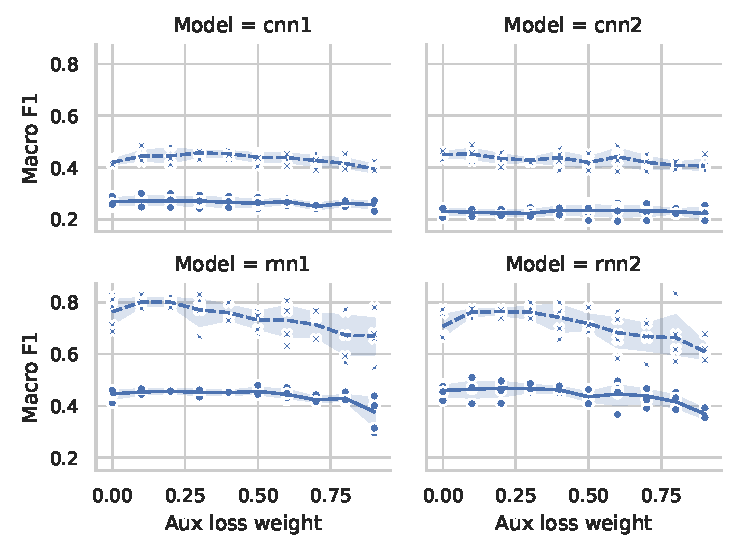
\includegraphics{lossweight}
  \caption[Performance of multi-task models]{
    Lines follow the mean of macro \FI scores. Shaded areas show 95\% confidence
    interval for the mean. Results for the collapsed set of classes are plotted with
    cross symbols and dashed lines.
  }
  \label{fig:lossweight}
\end{figure}

\todo{must check again}
The highest macro \FI scores on the full label set all come from RNN models.
The five highest scores range between $0.468$ and $0.483$ and were achieved
using auxiliary loss weights in the range from $0$ to $0.5$.
The highest macro \FI score in the previous chapter was $0.460$.


\todo{update figures}
\begin{figure}
  % cnn-multi-26199963_11
  \begin{subfigure}{\linewidth}
    \centering
    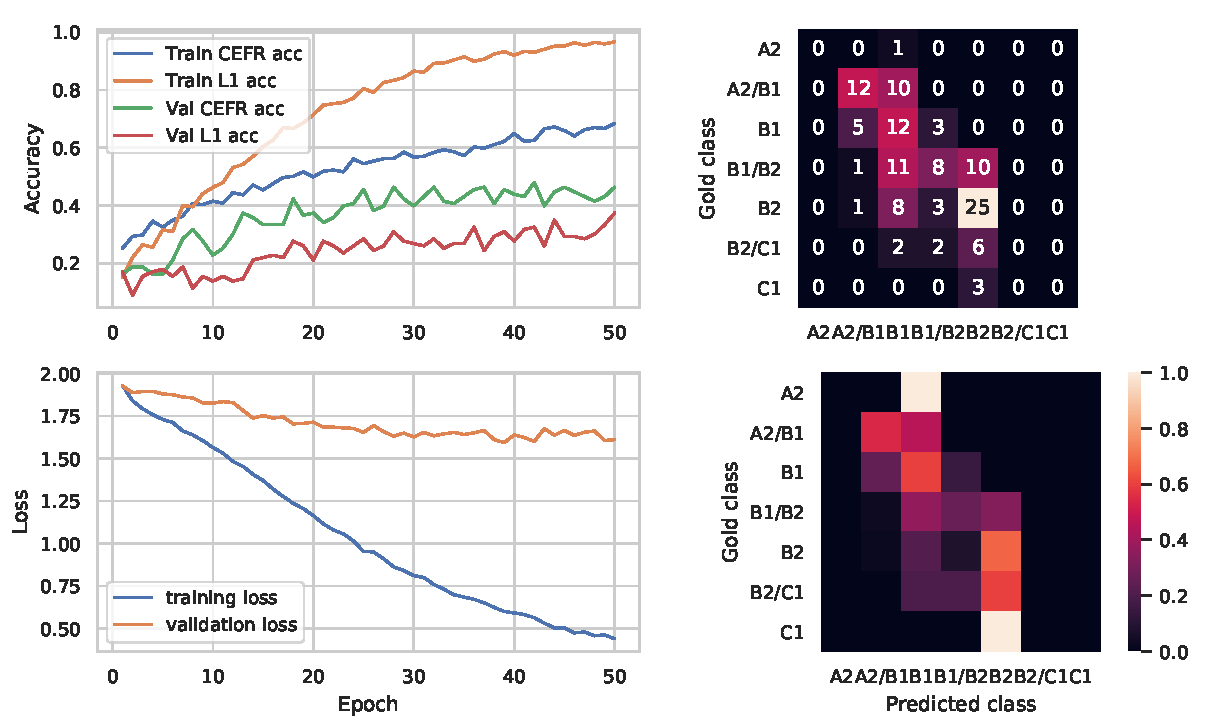
\includegraphics{cnn-multi-training}
    \caption{Training and validation loss and accuracy over 50 epochs of training.}
  \end{subfigure}
  \begin{subfigure}{\linewidth}
    \centering
    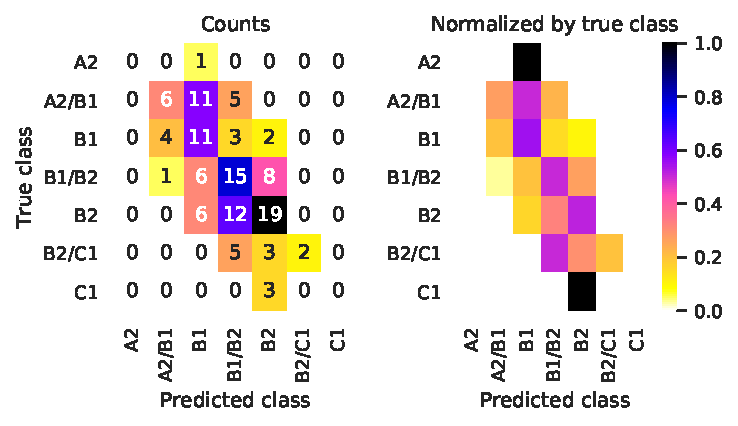
\includegraphics{cnn-multi-confusion}
    \caption{Confusion matrix on validation set, raw counts and normalized.}
  \end{subfigure}
  \caption{CNN2 0.75}
  \label{fig:cnn-multi-training}
\end{figure}

\begin{figure}
  % rnn-multi-26646843_28.pkl
  \begin{subfigure}{\linewidth}
    \centering
    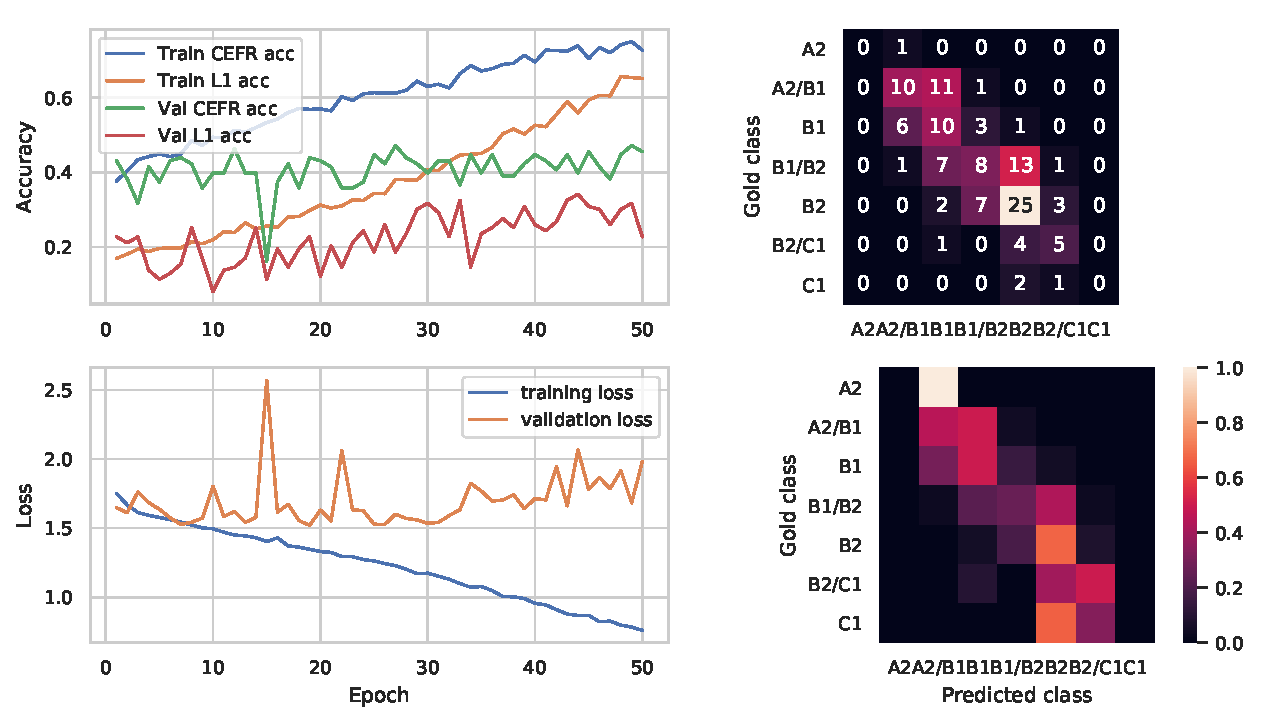
\includegraphics{rnn-multi-training}
    \caption{Training and validation loss and accuracy over 50 epochs of training.}
  \end{subfigure}
  \begin{subfigure}{\linewidth}
    \centering
    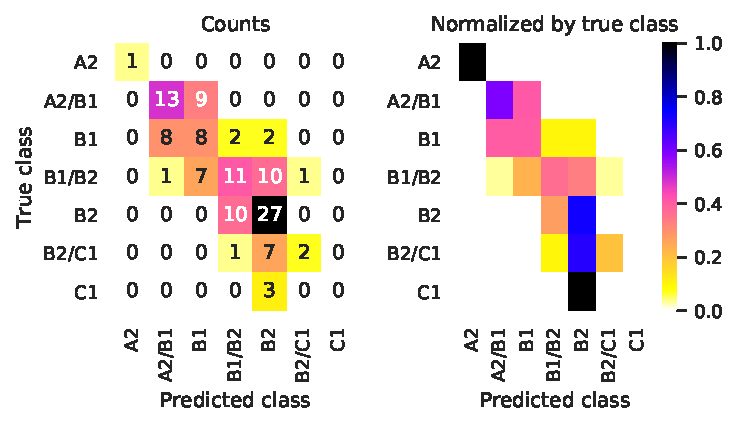
\includegraphics{rnn-multi-confusion}
    \caption{Confusion matrix on validation set, raw counts and normalized.}
  \end{subfigure}
  \caption{RNN1 0.5}
  \label{fig:rnn-multi-training}
\end{figure}


\section{Correlation of metrics}

\todo{More different metrics}

We have previously discussed different evaluation metrics. Since we now have
trained and evaluated a number of different models, it is possible to see
whether the metrics agree on the ranking of models.

\begin{figure}
  \centering
  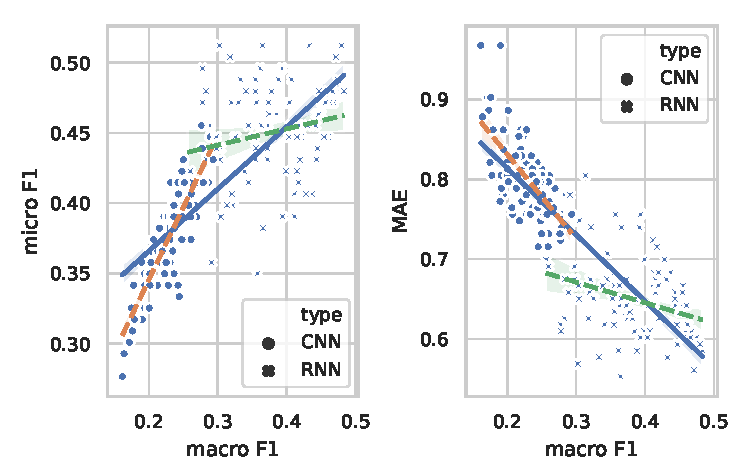
\includegraphics{reg_macro_F1_all}
  \caption[Macro \FI versus macro MAE]{
    Macro \FI versus macro MAE. Line of regression included in plot. The shaded
    area covers a 95\% confidence interval for the line of regression. CNN
    models are plotted with dots, RNN models with crosses.
  }
  \label{fig:reg_macro_F1_all}
\end{figure}

\begin{figure}
  \centering
  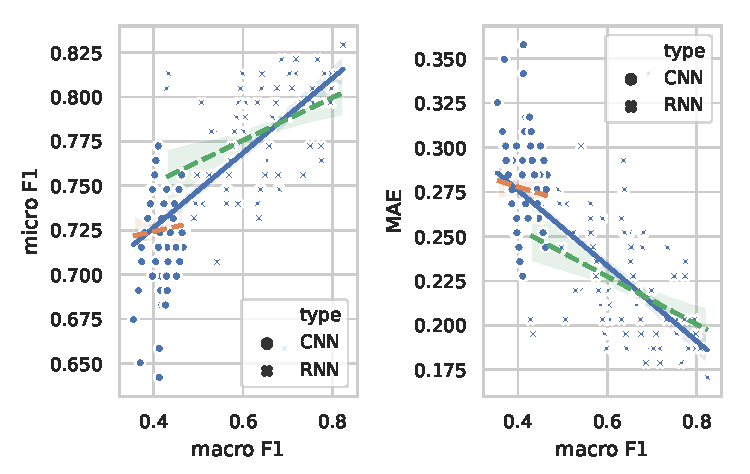
\includegraphics{reg_macro_F1_collapsed}
  \caption[Macro \FI versus macro MAE]{
    Macro \FI versus macro MAE for all experiments using collapsed CEFR labels.
    Line of regression included in plot. The shaded area covers a 95\%
    confidence interval for the line of regression. CNN models are plotted with
    dots, RNN models with crosses.
  }
  \label{fig:reg_macro_F1_collapsed}
\end{figure}

In figure \ref{fig:reg_macro_F1_all}, all experiments from this chapter have
been plotted to compare the macro \FI score to both the micro \FI score and
the macro mean average error.

The correlation is not all that strong, at least not for macro \FI vs. micro
\FI. Four experiments are tied for the highest micro \FI, but they range
between $0.302$ and $0.480$ in macro \FI.

It is also of note that the CNN and RNN experiments appear to form two
separate populations in the plot, with different correlation properties.
Table \ref{tab:metric-corrs} shows that in several cases, the correlation
value is much lower when examining CNN experiments and RNN experiments as
separate populations. \todo{Something with non-linearity} The correlation
values can be misleading when we combine two distinct populations into one
dataset. The most extreme case is the correlation between macro \FI and micro
\FI for collapsed CEFR labels. The CNN experiments are completely
uncorrelated, and the RNN experiments have a very low correlation coefficient
of $0.362$. Still, when combined, the correlation coefficient becomes
$0.721$.

In the other cases, while not as extreme, the Pearson coefficient is
significantly higher for CNN and RNN experiments together than for CNN and
RNN separately. The one exception is the correlation between macro \FI and
micro \FI for the full set of labels, where the CNN group has a higher
correlation coefficient on its own than when combined with the RNN
experiments. Notice also that in this case, the RNN experiments show no
correlation within their group.


\begin{table}
  \centering
  \begin{tabular}{lrrrr}
    \toprule
             & \multicolumn{2}{c}{Macro \FI vs. micro \FI}
             & \multicolumn{2}{c}{Macro F1 vs. macro MAE} \\
    \cmidrule(lr){2-3}
    \cmidrule(lr){4-5}
    Experiments & Correlation & $p$-value            & Correlation & $p$-value \\
    \midrule
      & \multicolumn{4}{c}{All CEFR labels} \\
    \midrule
    CNN         & $0.856$     & $7.02\cdot 10^{-30}$ & $-0.549$    & $3.34\cdot 10^{-9}$ \\
    RNN         & $0.196$     & $5.02\cdot 10^{-2}$  & $-0.780$    & $1.07\cdot 10^{-21}$ \\
    CNN+RNN     & $0.775$     & $2.39\cdot 10^{-41}$ & $-0.926$    & $1.05\cdot 10^{-85}$ \\
    \midrule
      & \multicolumn{4}{c}{Collapsed CEFR labels} \\
    \midrule
    CNN         & $0.055$     & $5.88\cdot 10^{-1}$  & $-0.331$    & $7.57\cdot 10^{-4}$ \\
    RNN         & $0.362$     & $2.15\cdot 10^{-4}$  & $-0.764$    & $2.48\cdot 10^{-20}$ \\
    CNN+RNN     & $0.721$     & $2.15\cdot 10^{-33}$ & $-0.941$    & $2.03\cdot 10^{-95}$ \\
    \bottomrule
  \end{tabular}
  \caption[Correlation of metrics]{
    Pearson's correlation coefficient between two pairs of evaluation metrics and
    different subsets of experiments. Two-tailed $p$-values are included.
  }
  \label{tab:metric-corrs}
\end{table}


The $p$-values reported for the correlation are to be taken with a grain of
salt. They were computed with the SciPy library \autocite{scipy}, which
states in its documentation other that the $p$-values should be reasonable
for datasets with at least 500 samples. The values in table
\ref{tab:metric-corrs} were computed on samples with either 100 or 200
samples, well below 500.
